\documentclass[10pt, conference, letterpaper]{IEEEtran}

\usepackage{algorithm}
\usepackage{algorithmicx}
\usepackage{algpseudocode}
\usepackage{amsfonts}
\usepackage{amsmath}
\usepackage{amssymb}
\usepackage[ansinew]{inputenc} 
\usepackage{xcolor}
\usepackage{mathtools}
\usepackage{graphicx}
\usepackage{caption}
\usepackage{subcaption}
\usepackage{import}
\usepackage{multirow}
\usepackage{cite}
\usepackage[export]{adjustbox}
\usepackage{breqn}
\usepackage{mathrsfs}
\usepackage{acronym}
%\usepackage[keeplastbox]{flushend}
\usepackage{setspace}
\usepackage{bm}
\usepackage{stackengine}
\usepackage[hidelinks]{hyperref}

\usepackage{listings}

\lstset{%
 backgroundcolor=\color[gray]{.85},
 basicstyle=\small\ttfamily,
 breaklines = true,
 keywordstyle=\color{red!75},
 columns=fullflexible,
}%

\lstdefinelanguage{BibTeX}
  {keywords={%
      @article,@book,@collectedbook,@conference,@electronic,@ieeetranbstctl,%
      @inbook,@incollectedbook,@incollection,@injournal,@inproceedings,%
      @manual,@mastersthesis,@misc,@patent,@periodical,@phdthesis,@preamble,%
      @proceedings,@standard,@string,@techreport,@unpublished%
      },
   comment=[l][\itshape]{@comment},
   sensitive=false,
  }

\usepackage{listings}

% listings settings from classicthesis package by
% Andr\'{e} Miede
\lstset{language=[LaTeX]Tex,%C++,
    keywordstyle=\color{RoyalBlue},%\bfseries,
    basicstyle=\small\ttfamily,
    %identifierstyle=\color{NavyBlue},
    commentstyle=\color{Green}\ttfamily,
    stringstyle=\rmfamily,
    numbers=none,%left,%
    numberstyle=\scriptsize,%\tiny
    stepnumber=5,
    numbersep=8pt,
    showstringspaces=false,
    breaklines=true,
    frameround=ftff,
    frame=single
    %frame=L
}

\renewcommand{\thetable}{\arabic{table}}
\renewcommand{\thesubtable}{\alph{subtable}}

\DeclareMathOperator*{\argmin}{arg\,min}
\DeclareMathOperator*{\argmax}{arg\,max}

\def\delequal{\mathrel{\ensurestackMath{\stackon[1pt]{=}{\scriptscriptstyle\Delta}}}}

\graphicspath{{./figures/}}
\setlength{\belowcaptionskip}{0mm}
\setlength{\textfloatsep}{8pt}

\newcommand{\eq}[1]{Eq.~\eqref{#1}}
\newcommand{\fig}[1]{Fig.~\ref{#1}}
\newcommand{\tab}[1]{Tab.~\ref{#1}}
\newcommand{\secref}[1]{Section~\ref{#1}}

\newcommand\MR[1]{\textcolor{blue}{#1}}
\newcommand\red[1]{\textcolor{red}{#1}}
\newcommand{\mytexttilde}{{\raise.17ex\hbox{$\scriptstyle\mathtt{\sim}$}}}

%\renewcommand{\baselinestretch}{0.98}
% \renewcommand{\bottomfraction}{0.8}
% \setlength{\abovecaptionskip}{0pt}
\setlength{\columnsep}{0.2in}

% \IEEEoverridecommandlockouts\IEEEpubid{\makebox[\columnwidth]{PUT COPYRIGHT NOTICE HERE \hfill} \hspace{\columnsep}\makebox[\columnwidth]{ }} 

\title{Ensembling CNN models for 3D Object Classification based on Voxel Grid representation}

\author{
    Simone D'Antimo$^\dag$, Harjot Singh$^\dag$, Jacopo Pegoraro$^\dag$
    \thanks{$^\dag$Department of Information Engineering, University of Padova,   \newline email: \texttt{\{simone.dantimo, harjot.singh\}@studenti.unipd.it,
    jacopo.pegoraro@unipd.it
    }}
    %\thanks{Special thanks to professor Jacopo Pegoraro}
} 

\IEEEoverridecommandlockouts

\newcounter{remark}[section]
\newenvironment{remark}[1][]{\refstepcounter{remark}\par\medskip
   \textbf{Remark~\thesection.\theremark. #1} \rmfamily}{\medskip}

\begin{document}

\maketitle
\begin{abstract}
\ac{CNN} have been widely used as Deep learning tools to enhance the spatial relationship among images and videos. In this paper, we illustrate the potential of CNN and Voxel grids for the 3D Object classification task. Intuitively, given a 3D image, we split it into blocks, each of those blocks may be only full or empty, which implies that the resolution of the 3D object is strongly correlated with the number of blocks in which they are split in, as trade-off more blocks implies more memory required for storage.
We decided to evaluate the potentiality and the limits of a 3D Object Classification System having a limited amount of computational capacity and memory storage: those limitations imply that we must use samples with a lower resolution (i.e. composed by a limited number of voxel), loosing some details and shape of the objects, but at the same time the results obtained show that we created a robust model which perform efficient analysis and can classify the objects independently of their rotation. We were able to reach good results on the test set, with an accuracy rate of 88 percent at the end.

\end{abstract}


\IEEEkeywords
Neural Networks, Convolutional Neural Networks, 3D Object Classification, Voxel Grid, ModelNet10, Data Augmentation.\endIEEEkeywords

\begin{figure*}[h]
\begin{center}
        \centering
        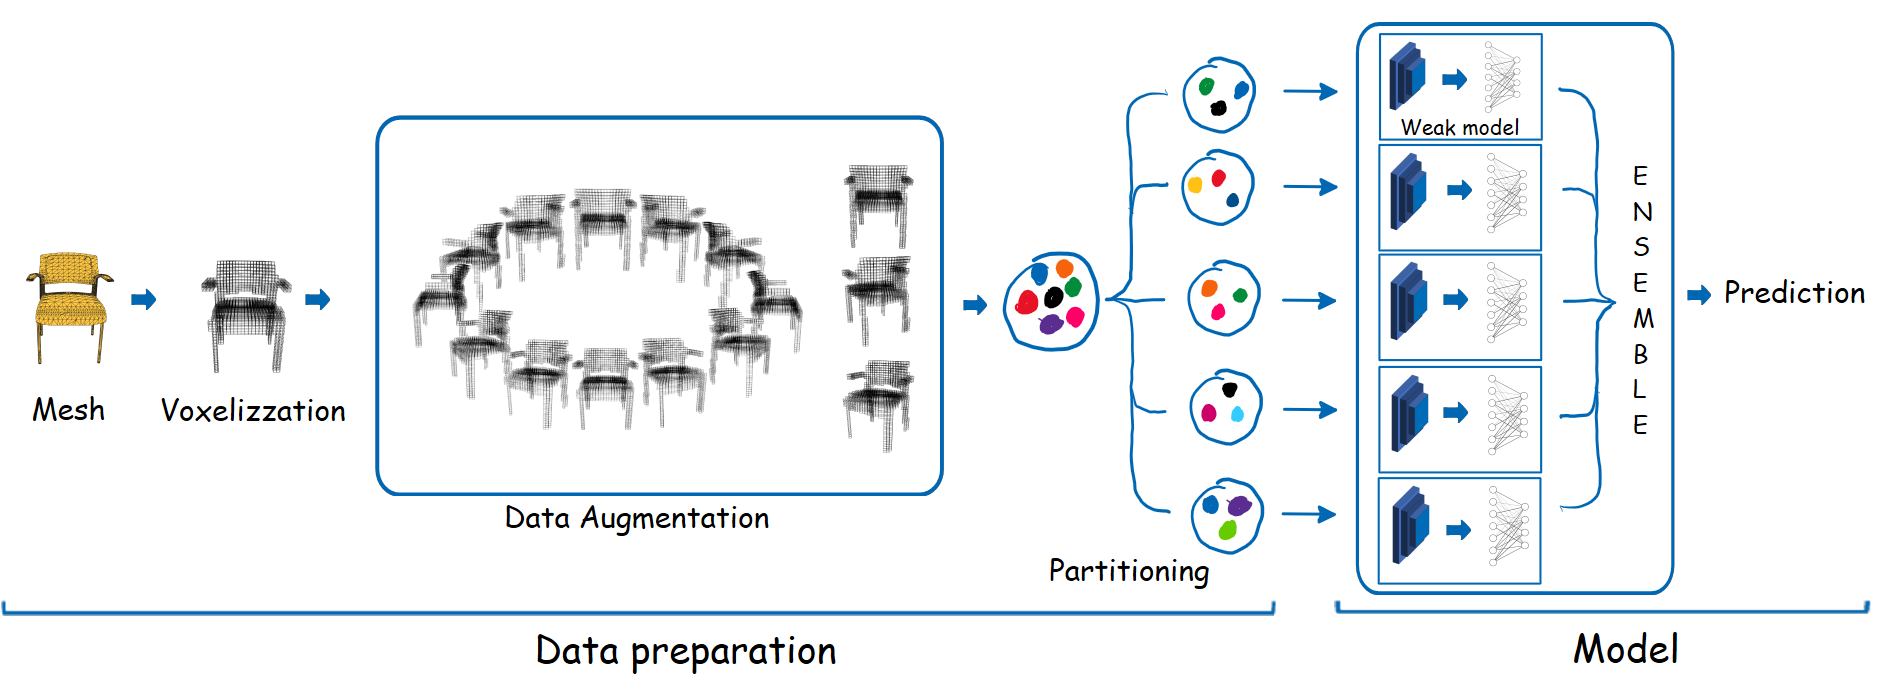
\includegraphics[width=\textwidth]{resources/pipeline.png}
        \caption{Processing Pipeline. Starting from left, we have the voxelization of the ModelNet10 dataset, followed by data augmentation with new rotations. Next, we have the partitioning of the rotated dataset into five different subsets. The subsets are give as input to the bagging models for the training.}
        \label{fig:pipeline}
    \end{center}
\end{figure*}

% !TEX root = template.tex

\section{Introduction}
\label{sec:introduction}

The 3D Object recognition task contributes to the field of computer vision by enabling the detection, classification and also localization of three-dimensional objects in images or video streams. Thanks to the improvements in Computer Vision and Deep Learning technologies these tasks are more and more reliable and accessible, enabling many emerging applications like augmented reality, virtual reality and many more related to robotics interactions with the environment. 
The way 3D data is represented has a significant impact on the performance of the 3D object detection. Here we introduce two of the most common representation for 3D Objects.
\begin{itemize}
    \item The Point-based representation uses a set of 3D points to describe the geometry of an object. This representation is lightweight and can handle large point clouds efficiently. The structure can  retain precise point positions, but at the same time it has a limited feature representation and since the points are unordered using them requires a high computational capacity \cite{liu2019pointvoxel}.

    \item Voxel-based representation models the object as a 3D grid of voxels, where each voxel has a binary value to indicate whether the object occupies it or not. This representation provides detailed information about the shape and structure of objects, but it requires a lot of memory, since we have to store also the empty blocks, therefore they are not scalable as other approaches \cite{liu2019pointvoxel}.
\end{itemize}

In this paper, we propose a "label predictor" that relies on 5 models using an ensembling technique to classify 3D objects, using at the same time a coarse voxel granularity. 
As mentioned above, the Voxel Grid structure maintains information regarding the shape and structure of the 3D Object, in order to properly capture and maximize the spatial relationship provided by the Voxel-Grid structure, we decided to use \ac{CNN}s as core networks. 

The main advantages of using this kind of approach is that each weak model is trained on a portion of the dataset, requiring smaller and thus quicker models. Since the weak models are trained on different portion of the dataset, they learn and make prediction based on different features, increasing the generalization of our ensemble system. If one can run all 5 weak models in parallel, and then choose the final label, this may result faster than running a single bigger model.

The memory requirements for voxelized 3D objects increase cubically with the resolution. We have seen that, for a resolution of 16, where each object is divided in a 16x16x16 voxel grid, the visualization is too coarse to be used. On the other hand, a resolution of 64 requires 262.400 blocks for each object, which is too much considering our memory capacity. In the end, we went with the resolution of 32x32x32, which has an affordable amount of blocks per objects ($\sim$32.000) \cite{liu2019pointvoxel}. In our case, this resolution is the optimal trade-off between memory and information loss. The expectation is that using a restrained number of blocks for each Object, the model will be more efficient by taking less time to execute and requiring less memory to storage all the Voxels information. 

The dataset which we used for training our models is a modified version of the ModelNet10 \cite{7298801}. The initial dataset is composed by 4899 aligned 3D CAD model divided in 10 different classes, we perform data augmentation to create a portion of rotated entries, which is useful to make our models learn how to classify objects independently of their rotation in the Z axis. 

The rest of the paper is organized as follows: Section \ref{sec:related_work} provides an overview of related works; Section \ref{sec:pipeline} describes our approach; In Section \ref{sec:dataset} we describe in details the dataset and pre-processing techniques; In Section \ref{sec:learning_framework} we present the Convolutional Neural Network that we built, summarizing the parameters we choose; In Section \ref{sec:results} we discussed our main findings; finally, Section \ref{sec:conclusions} draws some conclusions and outlooks for future works.\\


% !TEX root = template.tex

\section{Related Work}
\label{sec:related_work}

In recent times, object recognition has gained significant attention with the advancements in deep learning and computer vision technologies. These developments led to remarkable progress in the ability of computer systems to identify and recognize objects within images and videos. Many 3D Objects datasets are becoming free and accessible; Different deep learning models have been trained and tested on vast amounts of data and have exhibited good learning and generalization capabilities, surpassing the performance of traditional computer vision approaches. The generalization of the learned feature implies more capability to recognize an object even if it is rotated or is seen with a different angle, a paper that talks about this and create a model that may recognize an object regarding its orientation is "Orientation-boosted Voxel Nets for 3D Object Recognition" \cite{sedaghat2017orientationboosted}, they used pre-trained Convolutional Neural network from the VoxNet \cite{7353481} and re-trained to classify in addition also the rotations of the sample, this showed a clear improvement in the overall accuracy, going from 92\% to 93.9 on the ModelNet10 dataset.\\

In the corresponding field of 3D Object Detection, to overcome one of the challenges that may arise when using grid structures like voxels, namely capturing large context information in the structure itself.
In general, voxel grid solutions cannot capture large context information, which may be crucial for 3D object recognition and therefore classification. For large objects or particular objects, this may result in low accuracy.
State-of-the-art techniques in this field uses Transformer-based and Sparse CNN architectures and one of the relevant paper is Voxel Transformer for 3D Object Detection (VoTr) \cite{mao2021voxel}.
VoTr achieves cutting edge results by implementing both local and dilated attention mechanisms to capture both short and long-range context information by combining submanifold and Sparse modules.

These results can be replicated also in the 3D Object Classification field by integrating 3D CNN backbones like VoTr right before a Classification Network; Thinking about future works, also our model may benefit from incorporating techniques that are useful for capturing large amounts of context information as well.


Instead, with this paper, we propose different way to make the neural networks more independent and self continuous of the information on locality through Bagging and 3D cut-out techniques, and we will show an improvement on the overall accuracy on the task.

% !TEX root = template.tex
\begin{figure*}[h]
    \renewcommand\thefigure{\arabic{figure}.}
    \begin{center}
        \begin{subfigure}{0.45\textwidth}
            \centering
             \begin{subfigure}[b]{\textwidth}
                \renewcommand\thesubfigure{\alph{subfigure}.I}
                 \centering
                 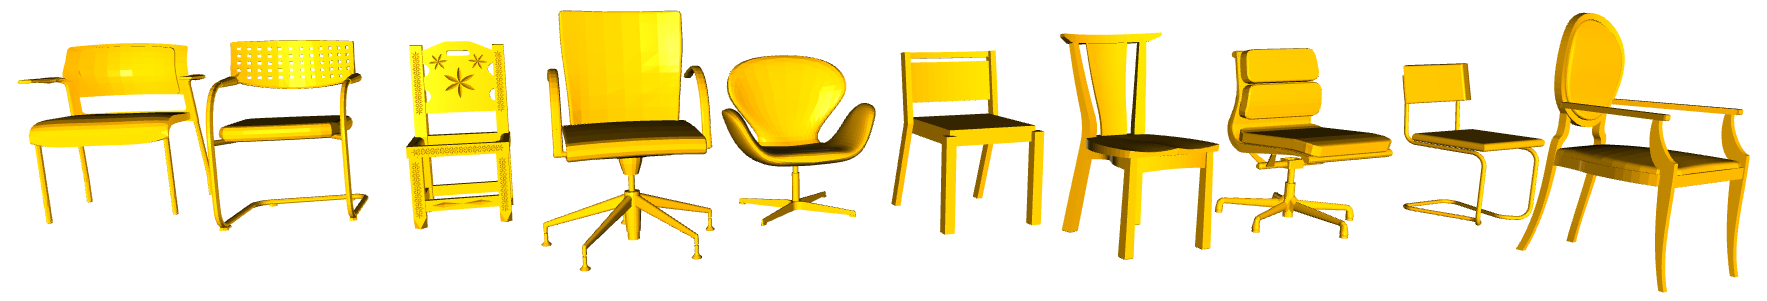
\includegraphics[width=\textwidth]{resources/chairs.png}
                 \caption{Chairs}
                 \label{fig:chairs}
             \end{subfigure}
             \begin{subfigure}[b]{\textwidth}
                \addtocounter{subfigure}{-1}
                \renewcommand\thesubfigure{\alph{subfigure}.II}
                 \centering
                 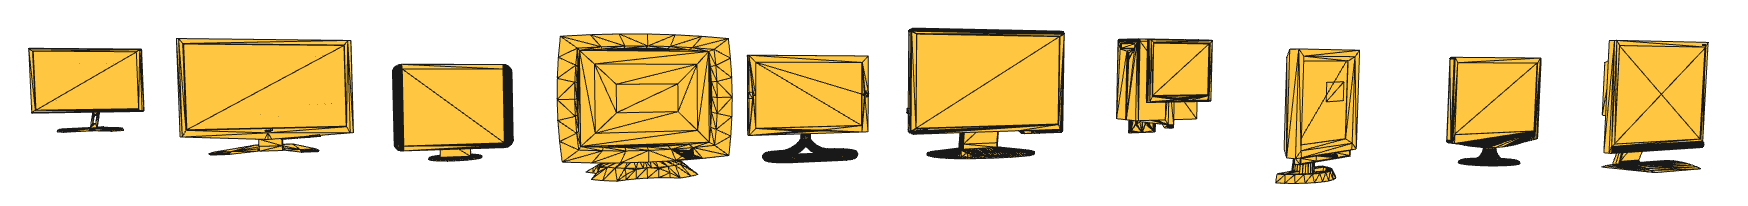
\includegraphics[width=\textwidth]{resources/monitor.png}
                 \caption{Monitors}
                 \label{fig:monitors}
             \end{subfigure}
            \addtocounter{subfigure}{-1}
            \caption{Example of (\ref{fig:chairs}) Chairs and (\ref{fig:monitors}) Monitors samples from \mbox{ModelNet10} dataset.}
            \label{fig:CADModels}
            \addtocounter{subfigure}{+1}
        \end{subfigure}
        \begin{subfigure}{0.10\textwidth}
        \end{subfigure}
        \begin{subfigure}{0.45\textwidth}
            %\renewcommand\thesubfigure{\alph{subfigure}.}
            \centering
             \begin{subfigure}[b]{\textwidth}
                \addtocounter{subfigure}{-1}
                \renewcommand\thesubfigure{\alph{subfigure}.I}
                 \centering
                 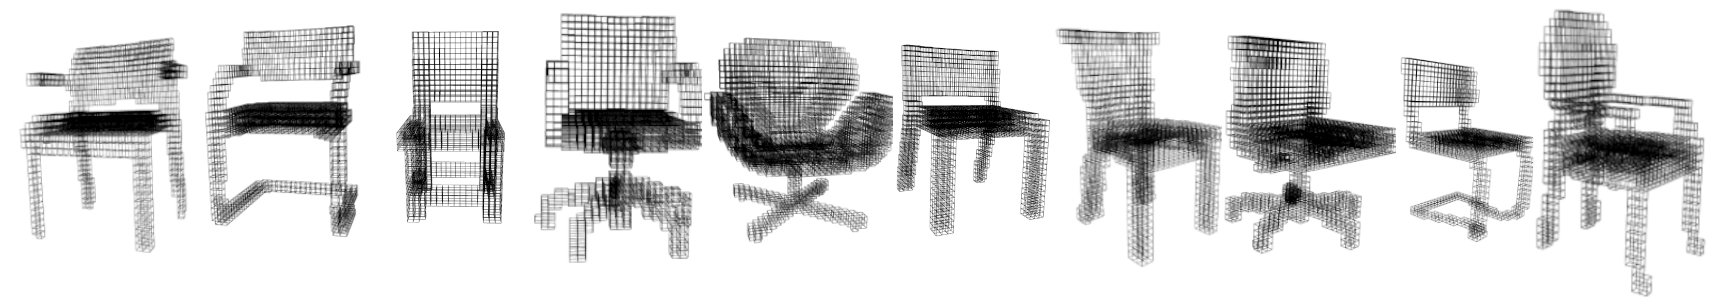
\includegraphics[width=\textwidth]{resources/chairs_voxels.png}
                 \caption{Chairs}
                 \label{fig:chairsVoxels}
             \end{subfigure}
             \begin{subfigure}[b]{\textwidth}
                \addtocounter{subfigure}{-1}
                \renewcommand\thesubfigure{\alph{subfigure}.II}
                 \centering
                 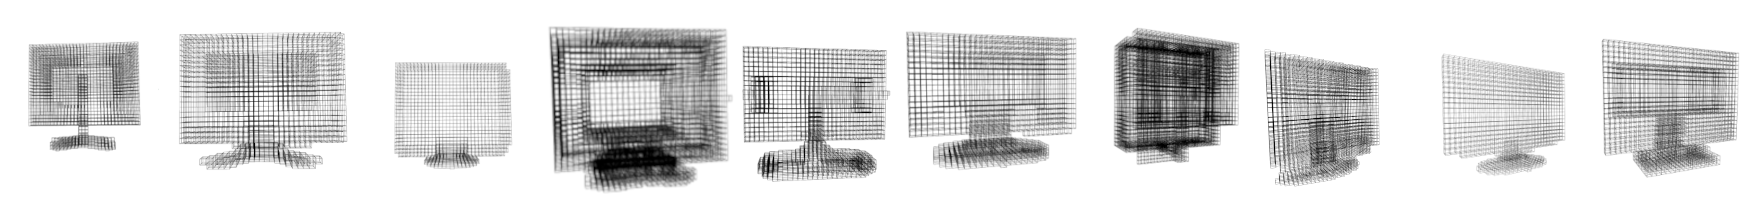
\includegraphics[width=\textwidth]{resources/monitors_voxels.png}
                 \caption{Monitors}
                 \label{fig:monitorsVoxels}
             \end{subfigure}
            \addtocounter{subfigure}{-1}
             
            \caption{Example of voxelized (\ref{fig:chairsVoxels}) Chairs and (\ref{fig:monitorsVoxels}) Monitors samples of Figure \ref{fig:CADModels}}
            \label{fig:VoxelizedModels}
        \end{subfigure}
        \caption{Examples of Chairs and Monitors samples. Fig.~\ref{fig:CADModels} shows the original CAD models, and Fig.~\ref{fig:VoxelizedModels} the voxelized versions of them.} 
        \label{fig:samples}
    \end{center}
\end{figure*}
\section{Processing Pipeline}
\label{sec:pipeline}

In this part, we explain our methodology, starting with the dataset preparation and giving some insights on our classifiers.\\

\textbf{Dataset preparation}
In the field of machine learning, the availability and quality of training data play a crucial role in determining the performance and generalizability of models. The original dataset we used as starting point, ModelNet10, comes as a clean collection of 3D CAD models for 10 classes of objects.
The owner has cleaned and manually aligned the orientations of the models, but they are not scaled nor \ac{IID}.

As the initial entries were CAD models, we had to translate them into voxel grids in order to use with 3D Neural Networks. 
%We used Open3d, a Python library, for the conversion, and then we normalized the grids.

To solve the unbalanced problem in the distribution of the samples, we choose to augment our data with Rotations. \\
%Fig.~\ref{fig:rotatedChair} shows an example of different rotations of the first chair in Fig.~\ref{fig:chairs}.
Rotations in our task has several advantages, e.g.: 
\begin{itemize}
    \item rotations helps our model to learn a stronger model that can recognize an object from different positions;
    \item data augmentation helps us to have more data to train our models;
    \item picking different number of rotations per category, depending on its initial distribution, we are able to balance the samples among the classes. More details in Sec. \ref{sec:dataset}.
\end{itemize}

%From Fig.~\ref{fig:finalTrainSetDistribution} we can see that the dataset becomes well-balanced with rotations.

%OLD: So we augmented the data with rotations, the methodology is explained in Sec. \ref{sec:dataset}, and using this approach we managed to arrive at a dataset with identically distributed classes.

We decided to store the rotated dataset efficiently as voxel grids, and start from this for the training. This allowed us to save a considerable amount of computation time, thus leaving only the transformation of those stored voxel grids into Binary Voxels (BV), required by the model.\\

Inspired by RandomErasing \cite{zhong2017random} and \cite{devries2017improved} , the cutout, 3d version of it, is applied to the sample during training. Cutout is a Data Augmentation technique which randomly masking out regions of the input data.
In our process, with a probability of 20\%, cutout removes a randomly selected 8x8x8 cube from the sample, by putting the voxel contained in this region to 0. This kind of technique encourage the network to learn more robust and general features and reduce overfitting. 
\\

\textbf{Models, Training and Evaluation}
As our baseline model for the classification, we started with a simple 3D CNN backbone followed by a fully connected layer. 
Initially, we choose to train the model on a smaller dataset to check if it was powerful enough to overfit, or we needed to increase the depth. Very soon the model overfitted it, thus we stick with the model for further improvements.\\
In order to make the model learn more general features, we used 3D Cut-Out technique, which improved the results of the baseline model.
The best result we get is with our bagging classifier, an ensemble of 5 baseline models trained on different partitions of the dataset. More details on partitioning in Sec.~\ref{sec:dataset} and on the classifier in Sec.~\ref{sec:learning_framework}.\\

Fig.~\ref{fig:pipeline} shows the training pipeline. We can see that for each weak model, we have a different partition, whereas during the evaluation phase, we used the test partition of the entire dataset.

%Then, we trained the 5 models that compose the bagging system on the entire dataset.
%We obtained 5 models, trained in different dataset, and at the end, we created a function which composes the predicted guess of all the 5 models to give as output the final prediction.

% TODO move to LF
%Each of the five weak classifier consists of two parts, 3D CNN backbone followed by a fully connected multi-layer neural network.

% Once we have obtained a Dataset of voxel grids we start the analysis and the creation of our models. The first thing we have to do is to read in memory the voxel from the dataset, each sample is represented as a list of coordinates of each non-empty voxel. We transform them into 3D boolean arrays of size 32x32x32 where each cell is true if and only if in such a position the associated voxel has a block on that grid. The spatial relationship is represented correctly with this data structure, but it increases the amount of memory required.


% Once the data are ready and in the correct shape what we need to do is to train our model. 
%We first tried to train our model with a smaller dataset to check if our network was powerful enough to overfit, or if we needed to increase the depth.
%Then, we trained the 5 models that compose the bagging system on the entire dataset.
%We obtained 5 models, trained in different dataset, and at the end, we created a function which composes the predicted guess of all the 5 models to give as output the final prediction.

  

% [TODO:https://arxiv.org/pdf/1901.08373.pdf:
% For the feature of every voxel, the simple
% Binary Voxel (BV) method is used to treat it as a binary value.
% The value 1 is assigned to the feature if there exists a point
% in corresponding voxel, otherwise, the voxel is empty and the
% feature value is 0. The drawback of this method is that the
% local shape information of points within a voxel is lost. To
% avoid the loss of local information, the voxel size in the BV
% is usually set very small to generate high-resolution 3D grids;

% An alternative method is to use PointNet [24] to extract the
% pointwise features, which is called Voxel Feature Encoding
% (VFE) [30]. It enables inter-point interaction within a voxel
% by combining pointwise features with a locally aggregated
% feature, which can help to learn the local 3D shape information, and hence, can alleviate information loss due to data
% quantization. Since VFE requires a number of points per valid
% voxel, the voxel size in VFE should be large. 
% ]

%Then we used a cutout technique to set a portion of size 8x8x8 to a determined number (20\%) of samples: Cutout is a Data Augmentation technique, one of the main benefits of Cutout is that it forces the model to learn to ignore irrelevant features in the input data, which can make the model more robust to unseen variations in the test data, but it can be a double-edged sword, so it must be used correctly otherwise it may reduce the performance of the model. Last we create and train our Convolutional neural network, it is composed by two Convolutional 3D layers, each of them followed by a Map Pooling, and the last two layers are dense, the output is an array of length 10, equal to the number of class in the dataset. 
%


\section{Dataset}
\label{sec:dataset}

In this section, we start by introducing the dataset used for our experiments, then explain how we processed it to use with our model, and finally how we made it an \ac{IID} dataset.
\ \\\\% INPUT DATA
\textbf{\ref{sec:dataset}.1. Input data} 

The dataset we used as starting point is ModelNet10, can be downloaded directly from \textit{https://modelnet.cs.princeton.edu/}. It contains 4899 3D CAD models divided into 10 different categories and has an initial splitting of the data into 80\% for training and 20\% for testing.
Fig.~\ref{fig:CADModels} shows some examples of chairs and monitors in the dataset.

% CAD Models
% \begin{figure}[h]
%     \begin{center}
%         \centering
%          \begin{subfigure}[b]{0.42\textwidth}
%              \centering
%              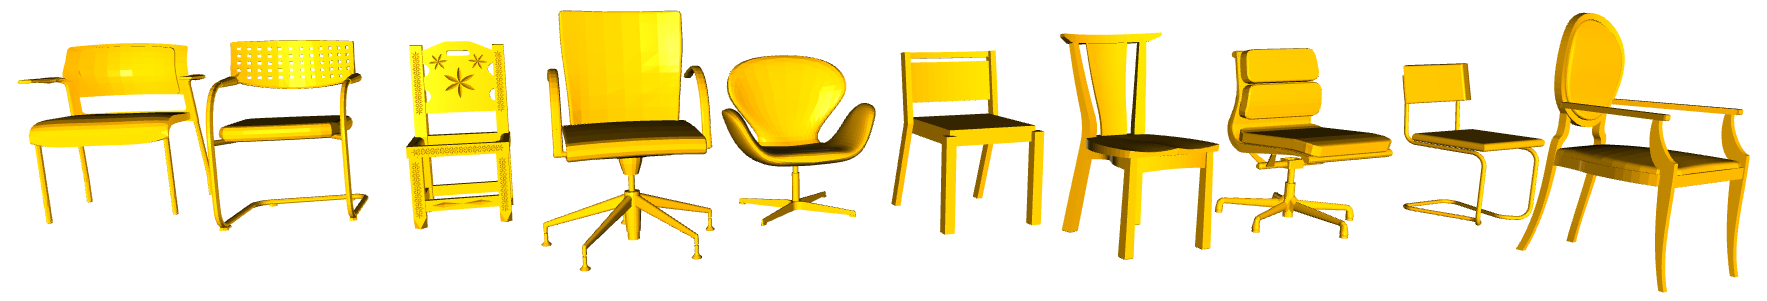
\includegraphics[width=\textwidth]{resources/chairs.png}
%              \caption{Chairs}
%              \label{fig:chairs}
%          \end{subfigure}
%          \begin{subfigure}[b]{0.42\textwidth}
%              \centering
%              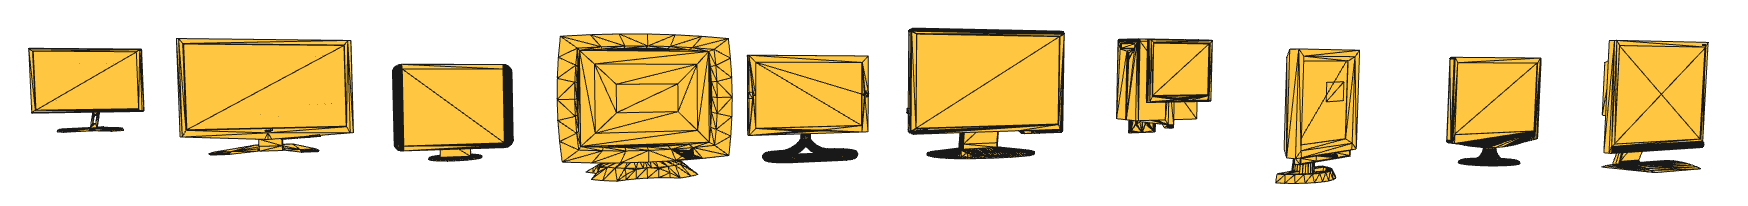
\includegraphics[width=\textwidth]{resources/monitor.png}
%              \caption{Monitors}
%              \label{fig:monitors}
%          \end{subfigure}
%         \caption{Example of (a) Chairs and (b) Monitors samples from ModelNet10 dataset.}
%         \label{fig:CADModels}
%     \end{center}
% \end{figure}
% % Voxelized Models
% \begin{figure}[h]
%     \begin{center}
%         \centering
%          \begin{subfigure}[b]{0.42\textwidth}
%              \centering
%              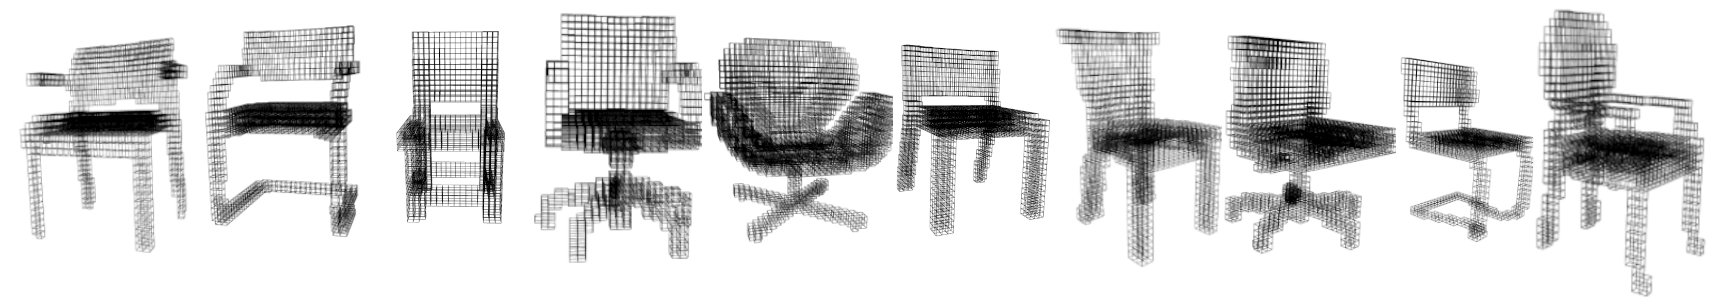
\includegraphics[width=\textwidth]{resources/chairs_voxels.png}
%              \caption{Chairs}
%              \label{fig:chairs}
%          \end{subfigure}
%          \begin{subfigure}[b]{0.42\textwidth}
%              \centering
%              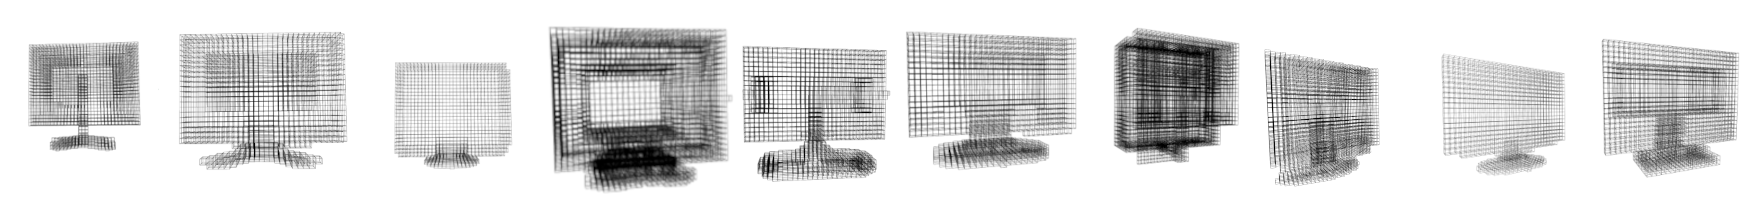
\includegraphics[width=\textwidth]{resources/monitors_voxels.png}
%              \caption{Monitors}
%              \label{fig:monitors}
%          \end{subfigure}
%         \caption{Example of voxelized (a) Chairs and (b) Monitors samples of Figure \ref{fig:CADModels}}
%         \label{fig:VoxelizedModels}
%     \end{center}
% \end{figure}
\ \\ % PRE-PROCESSING DATA
\textbf{\ref{sec:dataset}.2. Pre-processing data}

We had to solve mainly 2 problems with the initial dataset:
\begin{itemize}
    \item the samples were 3D CAD Models, so we needed to convert them into voxel grids for our needs;
    \item as we already mentioned, the Dataset is not \ac{IID}, so we decided to augment with rotations to make the categories well-balanced, Fig.~\ref{fig:finalTrainSetDistribution} in blue shows the initial dataset distribution of the Train folder.
\end{itemize}
%\ \\% 1)
\textbf{\ref{sec:dataset}.2.1. Voxelization}

The CAD models are Meshes, see Fig.~\ref{fig:CADModels} for reference, in Object File Format (OFF) but our model, described in the Sec.~\ref{sec:learning_framework}, requires 3D boolean vectors with dimensions of \mbox{$32\times32\times32$}.

With the help of the Open3d Python library \cite{Zhou2018}, we converted all the meshes into voxel grids after scaling them. 
% The code is available in our Git repository under the folder:  \mbox{\textit{code/preprocessing/voxelization/}}. \\
As mentioned before, voxel grids of size \mbox{$32\times32\times32$} are a good compromise between memory and information loss, and in our case we went from 2.17 GB of CAD models to 311 MB in voxelized version. 

Fig.~\ref{fig:VoxelizedModels} shows the voxelized samples of Fig.~\ref{fig:CADModels}.

We opted to store the normalized voxel grids directly on disk to reduce computation time during the training phase, as we relied only on the free tiers of GPU provided by Google Colab and Kaggle.\\
\ \\\\% 2)
\textbf{\ref{sec:dataset}.2.2. Data Augmentation}

The unbalanced distribution of the dataset may cause models to overfit classes with more samples, thus lowering the performances. 
Furthermore, in a real-world scenario, we found it very useful to consider that the model should be rotation-invariant, meaning that it can recognize objects regardless of their rotation.
Keeping in mind the above and the need to create a robust system, we choose to augment the data with new the rotation along the vertical axis. 

The rotations were made by adding multiples of 30 degrees to the initial orientation, thus in total we could have 12 possible rotations. Fig.~\ref{fig:rotatedChair} shows all the possible rotations of the first chair in Fig.~\ref{fig:chairs}.
% Rotated Models
\begin{figure}[h]
\begin{center}
        \centering
        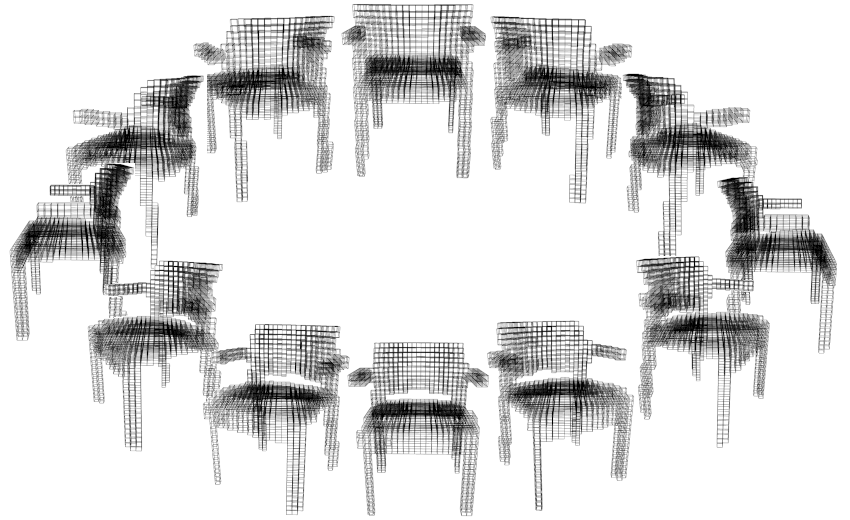
\includegraphics[width=0.42\textwidth]{resources/rotated_voxels_2.png}
        \caption{Example of possible rotation of the first Chairs in Figure \ref{fig:chairsVoxels}}
        \label{fig:rotatedChair}
    \end{center}
\end{figure}
In order to make the classes as equally distributed as possible, we choose uniformly at randomly N different rotations from all the possible ones. N values for each model in Train folder are described in Tab.~\ref{tab:modelRotations}. Meanwhile, we set N = 3 for the Test folder.

\begin{table}[h]
	\centering
	\caption{Categories and their N for Train partition, N is the total number of selected rotations}
	\label{tab:modelRotations}
	\begin{tabular}{|c||c|}
		\hline
		Rotations & Models \\
		\hline
		\hline
            2 & bed, chair, monitor, sofa\\\hline
            3 & table, toilet\\\hline
            5 & desk, dresser, night_stand\\\hline
            8 & bathtub\\\hline
	\end{tabular}
\end{table}

Fig.~\ref{fig:finalTrainSetDistribution} shows in orange the distribution after the Data augmentation.


% TODO: Also on Test set?
\begin{figure}[h]
\begin{center}
        \centering
        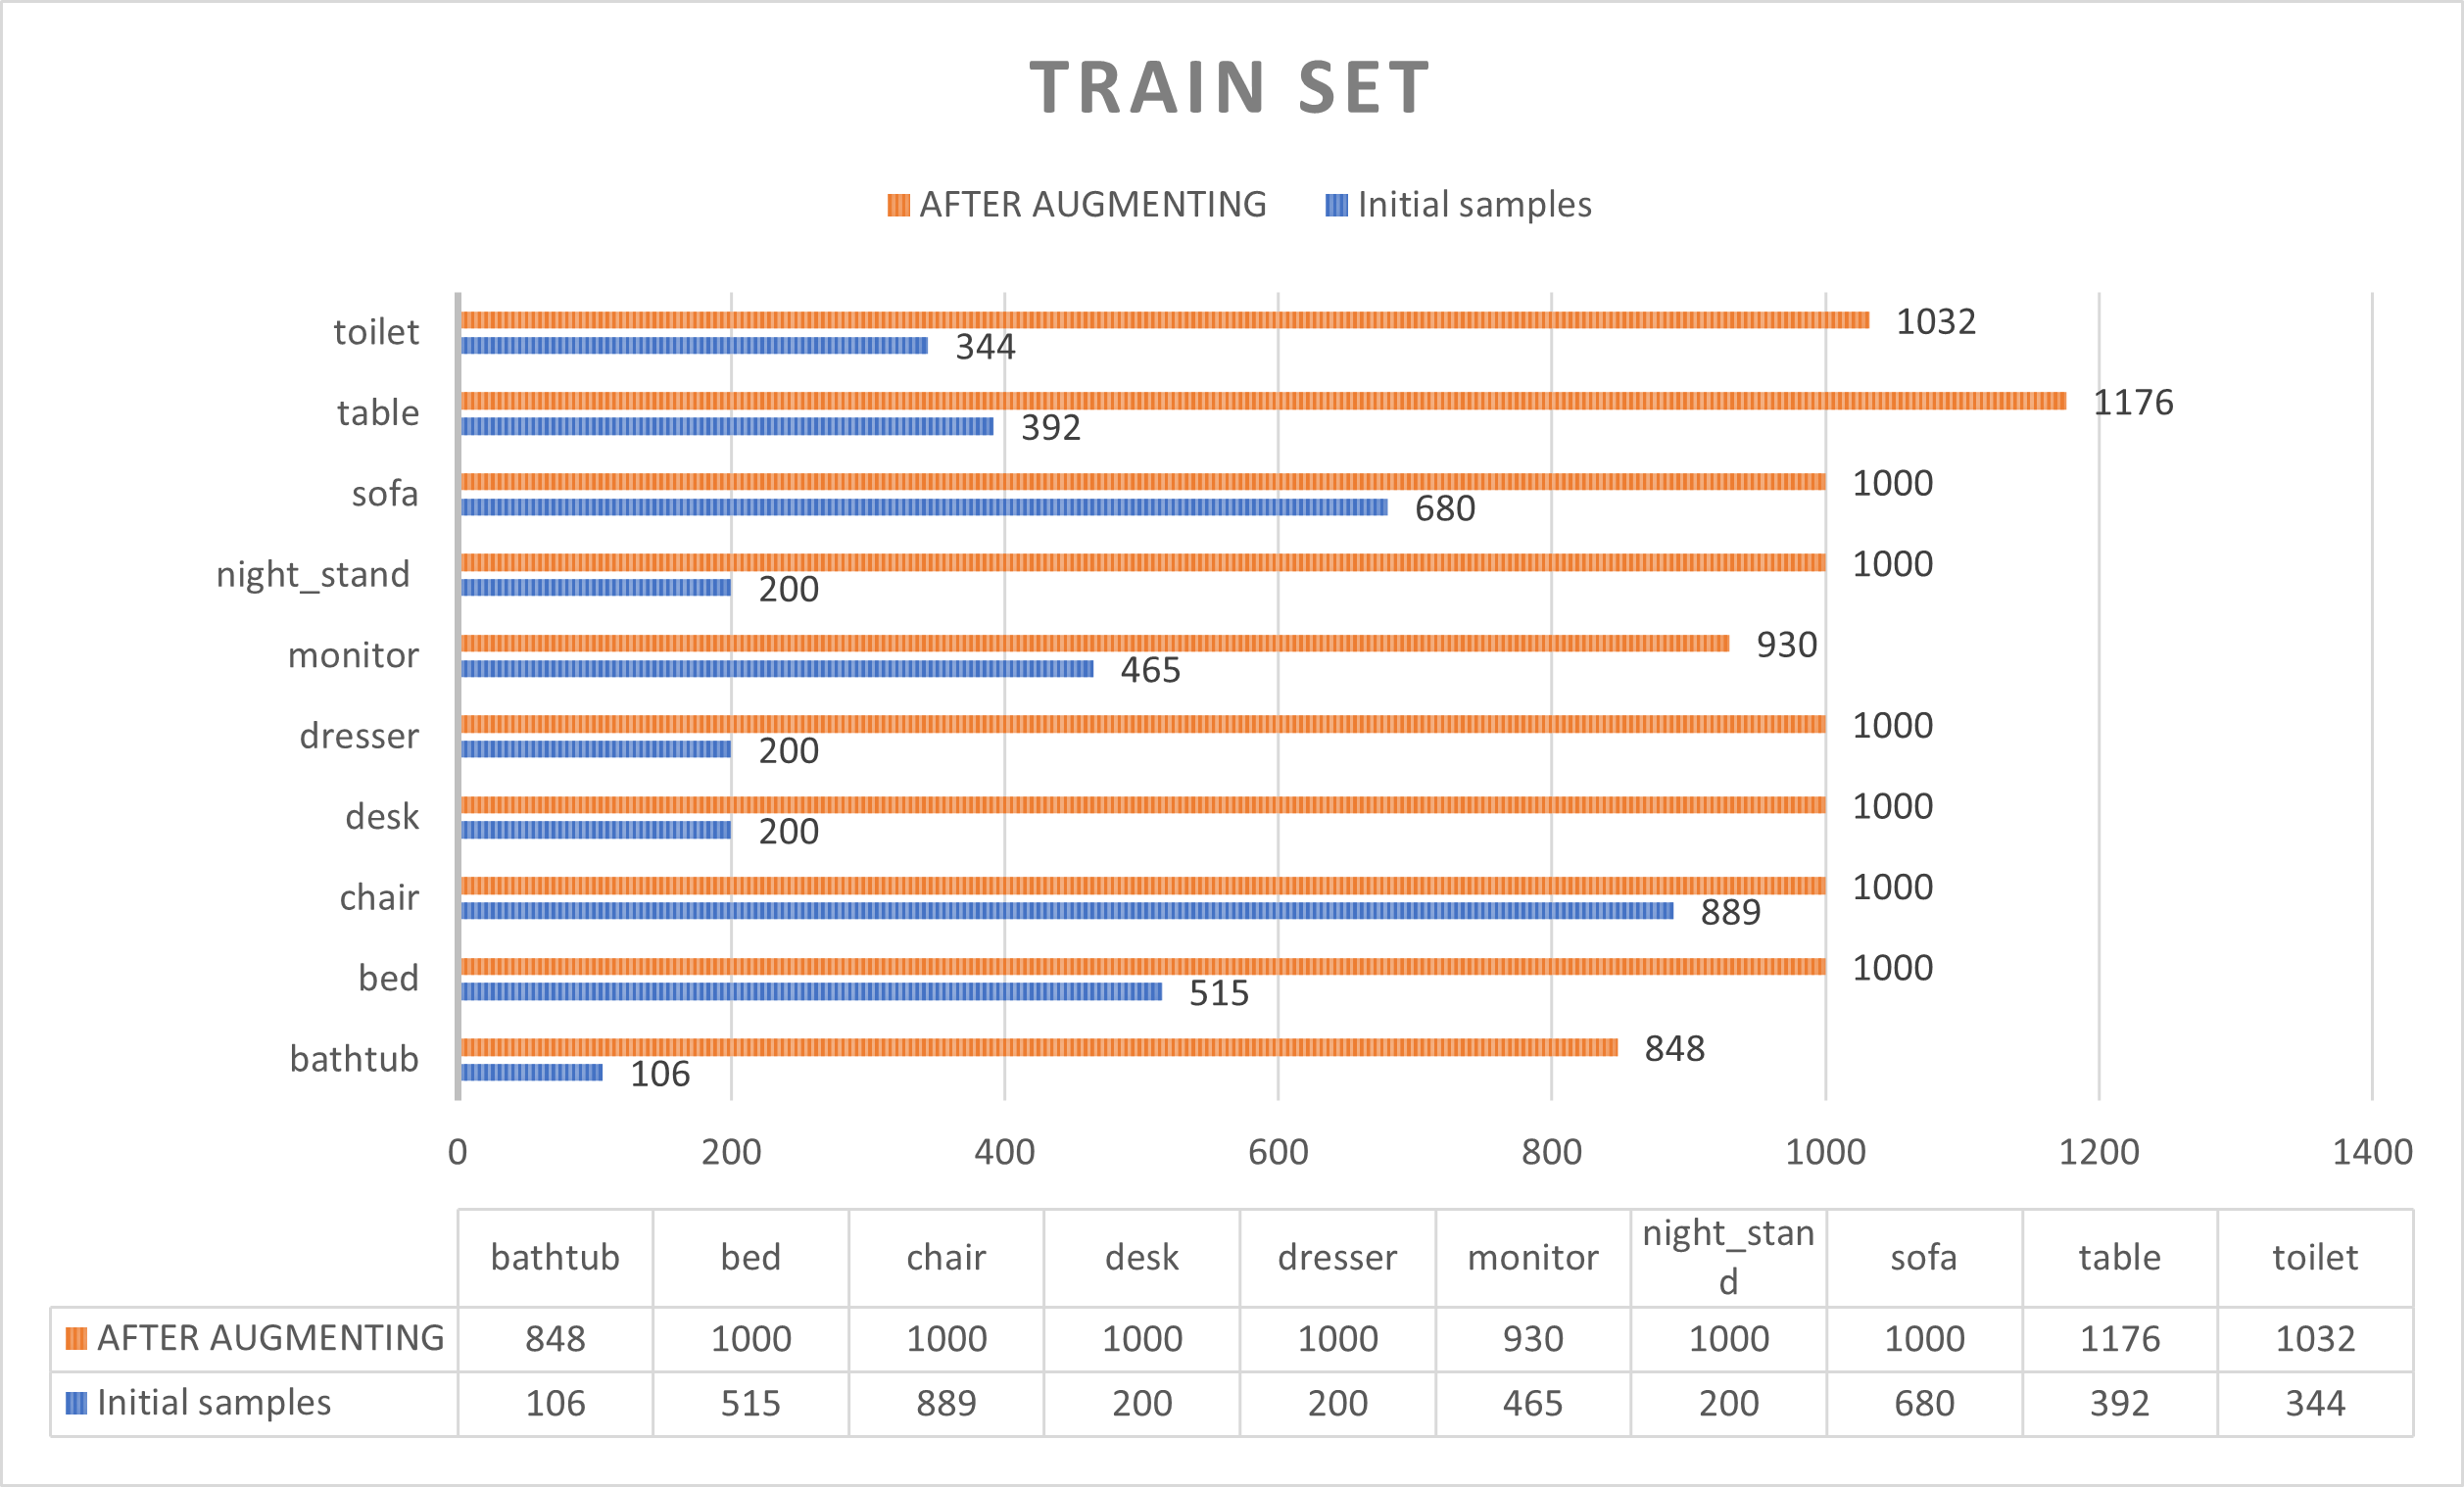
\includegraphics[width=0.42\textwidth]{resources/finalTrainDistribution.png}
        \caption{Distributions Before (in blue) and After (in orange) the data augmentation}
        \label{fig:finalTrainSetDistribution}
    \end{center}
\end{figure}

% As we can see from Figure \ref{fig:initialTrainSetDistribution}, the ModelNet10 is not an Independent and Identically Distributed (i.i.d.) dataset. The assumption of I.I.D is central to almost all machine learning algorithms, and we tried to make our data as much as i.i.d in the following way:
% \begin{itemize}
% 	\item Firstly, we normalized the data, from the previous step, by subtracting the mean and dividing by the standard deviation. [TODO: remove?]
% 	\begin{center}
% 		\textit{
% 			normalized\_voxelgrid = (voxelgrid - mean) / std
% 		}
% 	\end{center}
	
% 	\item Then, we augmented the dataset with new rotations of the voxel grids. Rotations are made by adding multiples of 30 degrees to the initial orientation. [TODO with formulas?]
	
% 	\item Finally, we randomly picked, per category, $\sim$1k samples for the train set and $\sim$300 samples for the test set. [TODO we are not precise here]
	
% \end{itemize}
% Figure \ref{fig:finalTrainSetDistribution} shows the distribution we get after these steps.
\ \\ % PARTITIONING DATA
\textbf{\ref{sec:dataset}.3. Partitioning data}

% A good practice is to divide the dataset into three sets: one set for training and two smaller sets for validation and testing.
% The ratio we used for splitting is 80/10/10, where 80 percent of the data is put into the training set, and the remaining percentage is equally spread across the test and validation sets.
To train the weak models for the bagging classifier, see Sec.~\ref{sec:learning_framework}, we created five different subsets with custom rules. 
The intention was to make each weak model :
\begin{itemize}
    \item learn well from their part of the dataset (chunk),
    \item also learn some information from the data of other models.
\end{itemize}

In details, we:
\begin{enumerate}
    \item Split tidily the rotated dataset into 25 subsets;
    \item Created 5 initial ordered chunks from the subsets;
    \item Copied each subset, of each chunk, into a different dataset w.r.t the initial chunk's dataset.
\end{enumerate}

 Tab.~\ref{tab:partitions} shows possible permutations for the datasets.

\begin{table}[h]
	\centering
	\caption{Our Bagging datasets compositions}
	\label{tab:partitions}
	\begin{tabular}{|c||c|c|}
		\hline
		Dataset & Chunk's subsets & Copied Subset \\
		\hline
		\hline
            1 & \small{01, 02, 03, 04, 05} & \small{10, 15, 20, 25 | 24}\\\hline
            2 & \small{06, 07, 08, 09, 10} & \small{01, 11, 16, 21 | 05}\\\hline
            3 & \small{11, 12, 13, 14, 15} & \small{02, 07, 17, 22 | 06}\\\hline
            4 & \small{16, 17, 18, 19, 20} & \small{03, 08, 13, 23 | 12}\\\hline
            5 & \small{21, 22, 23, 24, 25} & \small{04, 09, 14, 19 | 18}\\\hline
	\end{tabular}
\end{table}


\textbf{\ref{sec:dataset}.4. CutOut}

Finally, as explained in Chapter 3, we will perform the cutout on a portion of the dataset, masking out a random 8x8x8 portion of the input data. The probability that the cutout is applied to each sample is 20\%.


\section{Learning Framework}
\label{sec:learning_framework}
Bagging and boosting are ensemble techniques very used in machine learning context. Due to the limited resources, we only tried the Bagging, but we can expect similar results with Boosting. 

Our final classifier is based on bagging of 5 weak models to predict the class of the object.\\
Each of the five weak classifier consists of two parts:
\begin{itemize}
    \item The first part, that we called "3D Backbone", or simply a Convolutional Neural Network (CNN) module; %\ac{CNN}
    \item followed by a fully connected multi-layer neural network.
\end{itemize}
\ \\
\textbf{\ref{sec:learning_framework}.1. 3D Backbone}

In the 3D Backbone, the Input/Output of various layers remain shaped in 3 dimension, preserving spatial relationship. This part can be split into 3 similar blocks, each block is composed by 3D layer as presented in the Fig.~\ref{fig:blockDiagram}

\begin{figure}[h]
\begin{center}
        \centering
        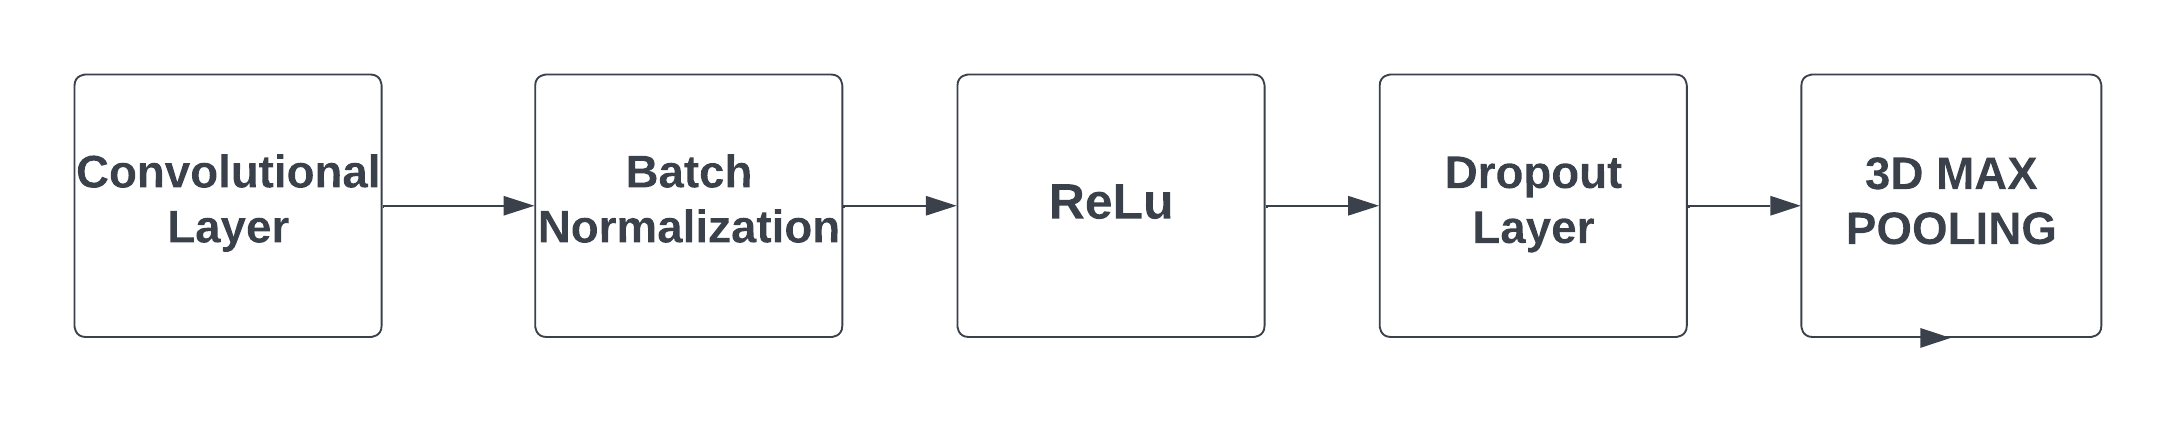
\includegraphics[width=0.5\textwidth]{resources/BlockDiagram.png}
        \caption{Single Layer of a 3D Backbone}
        \label{fig:blockDiagram}
    \end{center}
\end{figure}

The parameters for each of the block of the 3D backbone is reported in the Tab.~\ref{tab:conv-layers}.
We also test the Model with different learning rates and the one which seems to bring the best results was: Learning Rate = 1e-3.


\begin{table}[h]
\centering
\caption{Blocks of CNN 3D Backbone}
\label{tab:conv-layers}
\begin{tabular}{cccccc}
    \hline
    Block & Conv1 & Conv2 & Conv3 \\
    \hline
    Number of filters & 32 & 64 & 128 \\
    Kernel size & 3x3x3 & 3x3x3 & 3x3x3 \\
    Stride & 1 & 1 & 1   \\
    Padding & 1 & 1 & 1  \\
    Dropout ratio & 0.3 & 0.2 & 0.2  \\
    Max Pool Kernel & 2 & 2 & 2\\
    Max Pool Strides & 2 & 2 & 2\\
    Max Pool Paddings & 0 & 0 & 0\\
    \hline
\end{tabular}
\end{table}

\begin{table}[h]
    \centering
    \caption{Fully connected layers}
    \label{tab:fc-layers}
    \begin{tabular}{cccccc}
        \hline
        Layer & Fc1 & Fc2  \\
        \hline
        Number of Outputs & 128 & 10 \\
        Dropout ratio & 0.4 & 0.0   \\
        
        \hline
    \end{tabular}
\end{table}

\ \\
\textbf{\ref{sec:learning_framework}.1. FC network}

The second part of the weak model is composed by 2 fully connected layers. As is common for multi-class classification tasks, the output activation function in the final layer of our models is softmax.
\begin{equation}
    \sigma(\mathbf{z})_j = \frac{e^{z_j}}{\sum_{k=1}^{K}e^{z_k}}
\end{equation}
% \[
% \sigma(\mathbf{z})_j = \frac{e^{z_j}}{\sum_{k=1}^{K}e^{z_k}}
% \]
where
\begin{itemize}
    \item \textbf{z} represent the vector given in input to the softmax function
    \item z\textsubscript{j} the j\textsubscript{th} element of z
    \item \textbf{K} is the number of classes
\end{itemize}

Since the Convolutional backbone maintains the 3-dimensional shape of the object, in order to make the models make its prediction we flattened the output of backbone in a 1 dimension array, and given in input to the first Fully connected layer, which parameters are reported in the Tab.~\ref{tab:fc-layers}. The softmax function requires that the final output of the models has the number of outputs equal to the number of classes, and so it is.

The loss used for our models is the Cross-entropy loss, which is a common choice for multi-class classification tasks. It measures the dissimilarity between the predicted probability distribution by the softmax function and the true probability distribution of the target variable.
The Cross-entropy loss function has the following equations:
\begin{equation}
 L(p, y) = - (y * log(p) + (1 - y) * log(1 - p)) 
\end{equation}

Cross-entropy loss is calculated for each example in the training data, and the average loss over all examples is used as the final loss value.
We decided to run each of our model for 100 epochs, this choice was made to explore and capture the behavior of the models during the training phase, but how we will see in the next chapter, the models converges with less than 100 epochs.

The final result of the ensembled model is obtained by merging the prediction of all models, we tested two method to take the final prediction:
\begin{itemize}
    \item \textbf{Summing the Probabilities:} We sum the results of the softmax function from all the weak classifiers. The class with the highest sum of probabilities is then chosen as the final prediction. 
    \item \textbf{Voting:} In this method, each model in the ensemble makes its prediction, the final result is taken as the most voted class. 
\end{itemize}
    We tested both methodologies and in the end we decided to use the first approach, "sum the probabilities", for mainly two reasons, the first is that thanks to Softmax function we can explicit a sort of "belief" of correctness from a model, and we want to use this information for the final prediction, and the second reason is that having only 5 models it implies that the voting system may too easily end up in a tie, which may lead to uncertain results, e.g. 2 votes for class "bed", 2 votes for class "table", and 1 vote for class "bathtub". 
    
In the next chapter we will visualize and comment the results obtained


% !TEX root = template.tex

\section{Results}
\label{sec:results}

In this section, you should provide the numerical results. You are free to decide the structure of this section. As a general ``rule of thumb'', use plots to describe your results, showing, e.g., precision, recall and \mbox{F-measure} as a function of the system (learning) parameters. You can also show the precision matrix. 

\begin{remark}
Present the material in a progressive and logical manner, starting with simple things and adding details and explaining more complex findings as you go. Also, do not try to explain/show multiple concepts within the same sentence. Try to \textbf{address one concept at a time}, explain it properly, and only then move on to the next one.
\end{remark}

\begin{remark}
The best results are obtained by generating the graphs using a vector type file, commonly, either \texttt{encapsulated postscript (eps)} or \texttt{pdf} formats. To plot your figures, use the Latex \texttt{\textbackslash includegraphics} command. Lately, I tend to use pdf more.
\end{remark}

\begin{remark}
If your model has hyper-parameters, show selected results for several values of these. Usually, tables are a good approach to concisely visualize the performance as hyper-parameters change. It is also good to show the results for different flavors of the learning architecture, i.e., how architectural choices affect the overall performance. An example is the use of CNN only or CNN with adversarial training, or using residual layers for CNNs, dropout for better generalization or autoencoder models. So you may obtain different models that solve the same problem, e.g., CNN, CNN+residual layers, etc.
\end{remark}


% !TEX root = template.tex

\section{Concluding Remarks}
\label{sec:conclusions}
% What I would like to see here is:
% 1) a very short summary of what done,
% 2) some (possibly) intelligent observations on the relevance and applicability of your algorithms / findings,

The solution proposed in this paper provides a good accuracy, moreover we found  several advantages compared with a standard CNN model.

First, the memory requirements problem related to the Voxel grid is mitigated. 
%Since each weak model can be trained alone, we required to keep in memory only a portion of the dataset at a time. 
The solution implemented is very scalable, i.e. there are no specific constraints on the number of weak models, even if it's suggested to choose this number based on the availability of data. 

The execution of the whole system is also dynamic and can be adapted based on the potentiality of the computer in which it is executed. 
% 3) what is still missing, and can be added in the future to
% extend your work.
%In fact, since we use many small models that may run in parallel, the final prediction time may be lower than the amount of time required for the execution of a single bigger neural network. 
The model created can still be improved and enhanced using a larger number of models, and a larger dataset. 
Beyond enlarging the dataset and the number of models used for the final prediction for the Bagging, we can use another type of ensembling, i.e. Boosting. In our opinion, with Boosting we can further improve the results by paying more attention to wrongly classified classes like desk, dresser, night\_stand and table.
Furthermore, we would also like to explore the potential of sparse CNN \cite{graham2017submanifold} and transformers \cite{mao2021voxel} in classification task, to capture also long-range context information.\\
% 4 & 5 required by professor:
% Moreover: being a project report, I would also like to see
% a specific paragraph stating
% 4) what you have learned, and
% 5) any difficulties you may have encountered.
% This report showcases the work of the authors from the University of Padua on Project 3 (3D Objects Classification) of the Neural Network and Deep Learning Course.
% Our goal was to create a solution to classify Voxelized 3D objects, using Machine Learning techniques and ModelNet10 dataset as our reference.

During the development of this project we had possibility to develop the models on both, keras and pytorch, and we found that keras is much beginner-friendly than pytorch.
Another remark is that python libraries for 3D object manipulation are specialized for meshes and point clouds, but they don't provide full functionalities to work with voxel grid, we tested \textit{\href{http://www.open3d.org/}{open3d}} and  \textit{\href{https://trimsh.org/index.html}{trimesh}}, the popular ones. Even though Trimesh has more functions to work with voxels, the exportation of the voxel grids is not fully supported, so we used open3d for this project.
Finally, we trained our models on Colab and Kaggle, one of the free platforms that provide free GPU for the training, and we found that with colab is easier to connect with drive thus easier to comunicate between the notebook and drive itself for exchanging data. On the other hand, Kaggle provides different types of GPU and TPU. And for our bagging models, we trained the models in parallel, thus saving half of the training time.
% All the code is available in our Git repository at:  \mbox{\textit{\href{https://github.com/mrsingh-10/3d_classification}{https://github.com/mrsingh-10/3d\_classification}}}. \\

\acrodef{CNN}[CNN]{Convolutional Neural Networks}
\acrodef{IID}[i.i.d.]{Independent and Identically Distributed}

\bibliography{biblio}

\bibliographystyle{ieeetr}

\section{Individual Contribution}

- Simone D'Antimo: CutOut function, Bagging (and voting function), From list of Voxel to Voxel-Grid function, first tries with the CNN models (Keras), Fine-tune of the CNN parameters.

- Harjot Singh: 
Voxelization of CAD models, Data Augmentation with Rotations, Adaptation from Keras to Pytorch, Fine-tune of the CNN parameters, implementation of ORION neural network, managed the workflow and front end of the final notebooks (Colab and Kaggle).

We both equally contributed to all the sections of the report. We both help each other to perform the relative tasks.

\end{document}


